\section{Project Design}
% Include class diagrams and reasonings of the design
\label{sec:project-design}
\begingroup
\sloppy

\subsection{Scope and Architectural Objectives}

The Mario Game Project is a C++17, SFML-based two-dimensional platformer.  It
supports three selectable heroes, three selectable levels, data-driven Tiled
maps, multiple hero forms, enemy AI, a multi-phase boss, blocks and power-ups,
hero and enemy projectiles, sound, a HUD, pause/save/continue flows, and victory
or defeat transitions.  The design has four primary objectives:

\begin{enumerate}
    \item keep application navigation separate from gameplay simulation;
    \item construct levels and entities from map or save data rather than in
    the main loop;
    \item represent behavior through polymorphism and composition so new
    characters, states, entities, and levels can be added locally; and
    \item make ownership explicit through RAII smart pointers, with narrow
    non-owning callbacks for cross-system events.
\end{enumerate}

The implementation is organized into the \texttt{Core}, \texttt{Gameplay},
\texttt{Entities}, \texttt{Managers}, and \texttt{Utilities} areas.  SFML
provides the window, events, timing, graphics, views, textures, text, and audio.
Tiled \texttt{.tmj} maps are parsed with the vendored nlohmann JSON library.

\subsection{High-Level Architecture}

At the highest level, \texttt{Game} runs a fixed-step application state stack.
\texttt{PlayingState} is the presentation-level controller for an active game,
while \texttt{LevelRuntime} is the gameplay facade.  The latter owns the world
and delegates physical movement and entity interactions to dedicated systems.

\begin{figure}[htbp]
\centering
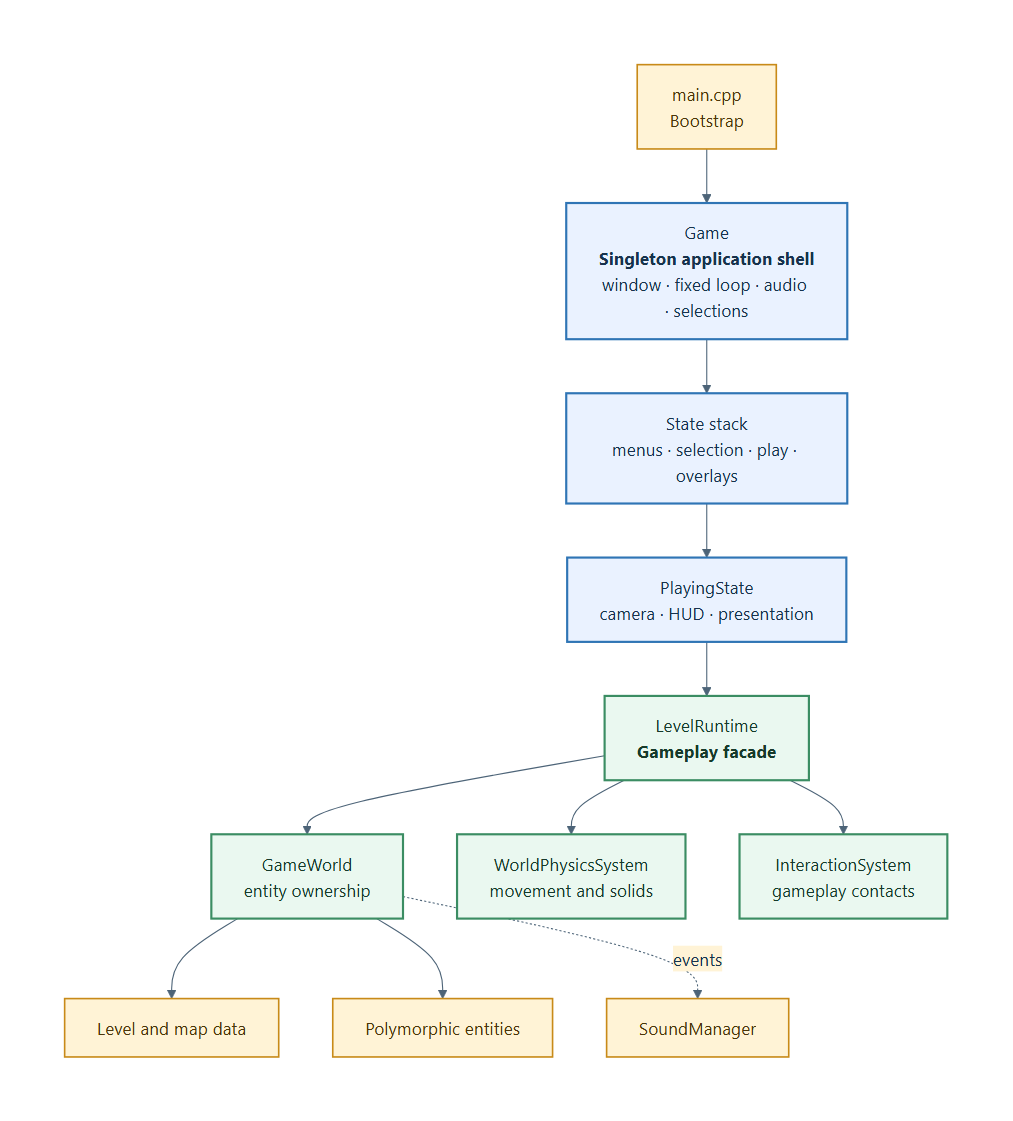
\includegraphics[width=0.76\textwidth,height=0.68\textheight,keepaspectratio]{img/diagrams/project-overall-architecture.png}
\caption{Layered runtime architecture of the game.}
\label{fig:overall-architecture}
\end{figure}

\begin{table}[htbp]
\centering
\small
\renewcommand{\arraystretch}{1.2}
\begin{tabular}{|p{0.19\textwidth}|p{0.33\textwidth}|p{0.37\textwidth}|}
\hline
\textbf{Area} & \textbf{Main abstractions} & \textbf{Responsibility} \\
\hline
Application shell & \texttt{Game}, \texttt{State} and concrete screen states & Window and fixed loop, event dispatch, screen navigation, overlays, global selection and audio lifetime. \\
\hline
Gameplay facade & \texttt{PlayingState}, \texttt{LevelRuntime} & Camera/HUD and transitions on one side; ordered simulation and region/pipe behavior on the other. \\
\hline
World and systems & \texttt{GameWorld}, \texttt{LevelBuilder}, \texttt{WorldPhysicsSystem}, \texttt{InteractionSystem} & Entity ownership, initial construction, terrain collision, entity-to-entity rules, and cleanup. \\
\hline
Domain entities & Characters, blocks, items, projectiles, goals & Polymorphic gameplay behavior and rendering. \\
\hline
Data/services & Map, level, save, HUD and sound managers & Parse and render map data, persist sessions, display metrics, and play audio. \\
\hline
Utilities & \texttt{Animator}, physics constants, shared Thunder Flash texture & Reusable animation, tuning constants, and lazy texture processing. \\
\hline
\end{tabular}
\caption{Primary architectural areas and responsibilities.}
\end{table}

\subsection{Overall Class Diagram}
\label{subsec:overall-class-diagram}

Figure~\ref{fig:overall-class-diagram} summarizes the main static relationships
across the complete project.  The application layer owns polymorphic screen
states and long-lived services.  The active \texttt{PlayingState} owns one
\texttt{LevelRuntime}, which acts as the facade over world data, physics, and
semantic interactions.  \texttt{GameWorld} is the aggregate root for live
entities, while heroes and enemies delegate their changing behavior to form and
state objects.  Builders and managers remain outside the entity hierarchies so
that construction, persistence, and presentation do not become entity concerns.

\begin{figure}[p]
\centering
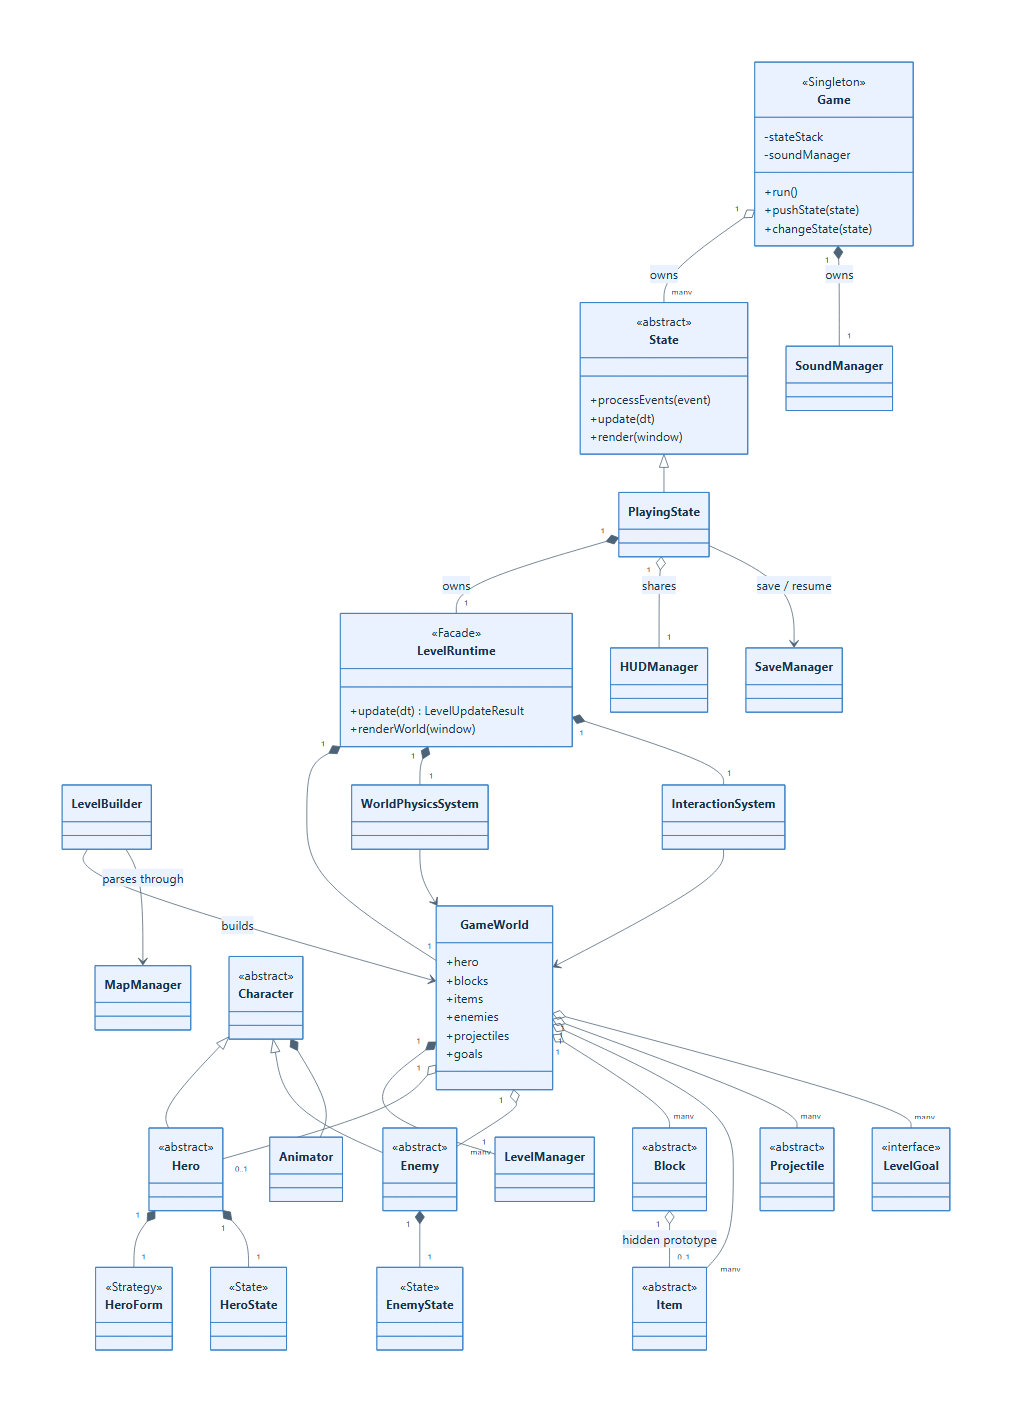
\includegraphics[width=0.94\textwidth,height=0.82\textheight,keepaspectratio]{img/diagrams/project-overall-class.png}
\caption{Overall class diagram of the application shell, gameplay facade,
world ownership, domain entities, and supporting services.}
\label{fig:overall-class-diagram}
\end{figure}

The diagram deliberately shows architectural classes and families rather than
every concrete subclass.  The focused diagrams in the following subsections
expand the screen, hero, enemy, block, item, projectile, goal, and service areas.

\subsection{Application Bootstrap, Main Loop, and State Stack}

\subsubsection{Bootstrap and resource lifetime}

\texttt{src/main.cpp} is intentionally small.  It obtains the singleton
\texttt{Game}, queues a \texttt{MainMenuState}, and calls \texttt{run()}.
\texttt{Game} owns the only \texttt{sf::RenderWindow}, the state stack, the
long-lived \texttt{SoundManager}, selected hero and level metadata, and global
volume settings.  On Windows, \texttt{main.cpp} also contains a compatibility
definition for legacy standard-I/O symbols required by the linked environment.

The loop uses a fixed simulation step of $1/60$ second and a variable render
rate.  Elapsed wall time is clamped to $0.25$ seconds before it is accumulated.
This cap is important when a large map or texture takes time to load: the game
does not spend many seconds replaying accumulated fixed updates after the load.
Events are polled during fixed updates, the active state is updated, and the
visible portion of the state stack is rendered once per outer loop iteration.

State transitions are deferred.  A state may request Push, Pop, Replace, or
Clear-and-Push, but \texttt{Game::applyPendingStateAction} commits the request
outside the state's callback.  This prevents deletion of a state while its own
event or update function is executing.  Repeated Tab and Enter key-press events
are filtered until their key-release events, preventing duplicate activations.

\subsubsection{Screen-state class diagram}

\begin{figure}[htbp]
\centering
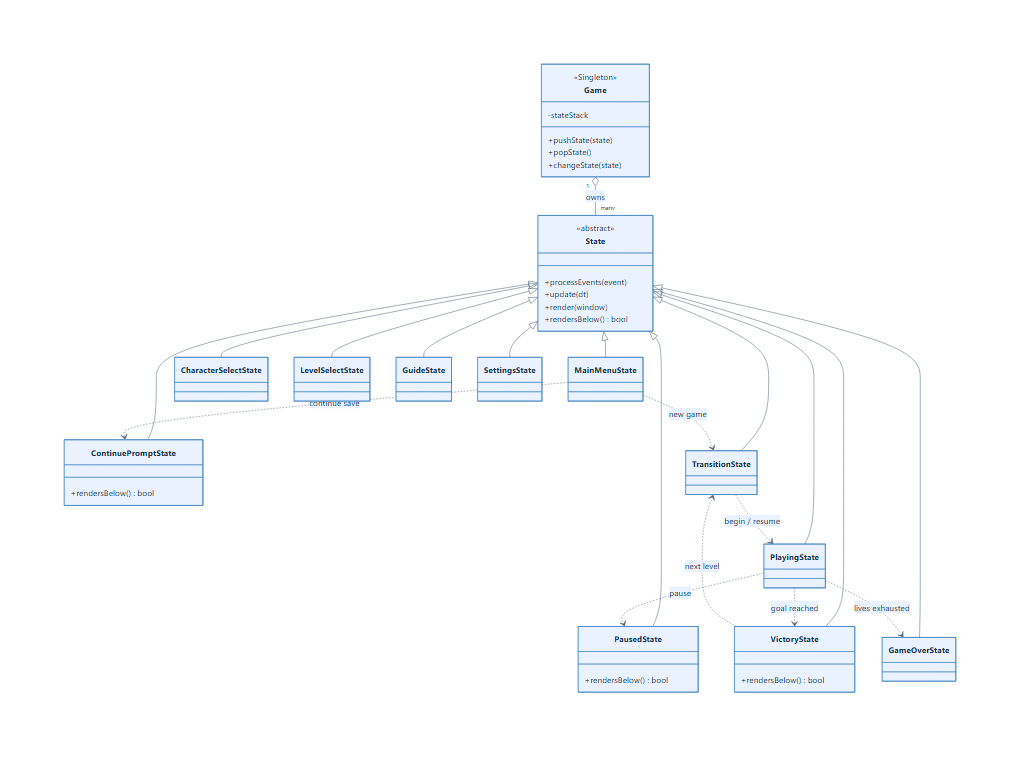
\includegraphics[width=0.98\textwidth,height=0.68\textheight,keepaspectratio]{img/diagrams/project-screen-states.png}
\caption{Application state hierarchy and principal navigation paths.}
\label{fig:screen-state-diagram}
\end{figure}

\subsubsection{Responsibilities of each screen}

\begin{description}
    \item[\texttt{MainMenuState}] Presents Play, Character, Level, Guide, and
    Settings buttons.  Play opens \texttt{ContinuePromptState} if an existing
    save is found; otherwise it starts a transition directly.  The menu also
    displays the currently selected world and starts menu background music.

    \item[\texttt{ContinuePromptState}] Is a modal overlay
    (\texttt{rendersBelow()} is true).  It validates the save's map and tileset,
    resolves its catalog/world labels, and offers Continue or New Game.
    Continuing restores HUD metadata and enters \texttt{TransitionState} with
    a resume flag; New Game clears the stack and uses current selections.

    \item[\texttt{CharacterSelectState}] Displays Mario, Luigi, and Flash cards.
    Confirmation writes a \texttt{HeroType} into \texttt{Game} and returns to
    the menu.  It does not construct the hero; construction is deferred until
    a level is built.

    \item[\texttt{LevelSelectState}] Builds its three cards from
    \texttt{LevelCatalog::LEVELS}.  Levels 1, 2, and 3 correspond to worlds
    1-1, 1-2, and 1-3 and are currently marked \texttt{READY}.  Confirmation
    stores the map path and world label in \texttt{Game}.

    \item[\texttt{GuideState}] Implements a paged help screen with character,
    item, and keyboard/control illustrations.

    \item[\texttt{SettingsState}] Owns two reusable slider records for BGM and
    SFX volume.  Keyboard, mouse, hover, and drag operations update the global
    \texttt{Game} settings and therefore the live \texttt{SoundManager}.

    \item[\texttt{TransitionState}] Displays the selected world and remaining
    lives for two seconds, then replaces itself with \texttt{PlayingState}.  A
    shared \texttt{HUDManager} survives retries and next-level transitions.

    \item[\texttt{PlayingState}] Owns camera and HUD presentation, one
    \texttt{LevelRuntime}, pause/save integration, level theme music, victory
    and defeat delays, and Thor King phase-three environmental effects.

    \item[\texttt{PausedState}] Is a modal overlay containing Resume, Save, and
    Main Menu commands.  The Save command invokes a callback supplied by the
    underlying \texttt{PlayingState}; the pause state therefore does not need
    access to the complete world.

    \item[\texttt{VictoryState}] Is a modal animated overlay offering Replay,
    Main Menu, and Next Level.  Next Level uses
    \texttt{LevelCatalog::nextAfter}, preserves the shared HUD, resets the
    timer, updates the selected level, and enters another transition.

    \item[\texttt{GameOverState}] Presents the defeat animation and returns to
    the menu when Enter is pressed.
\end{description}

This state hierarchy is preferable to a single screen-mode switch in the main
loop.  Every screen owns only its own graphical controls and input rules, while
\texttt{Game} supplies one uniform lifetime and navigation protocol.

\subsection{Gameplay Coordination and World Ownership}

\subsubsection{Facade and subsystem boundaries}

\texttt{PlayingState} is intentionally not the owner of entity collections.
It delegates them to \texttt{LevelRuntime}, which provides a facade over the
complete running level.  \texttt{LevelRuntime} in turn owns
\texttt{GameWorld}, \texttt{WorldPhysicsSystem}, and
\texttt{InteractionSystem}; it creates a short-lived \texttt{LevelBuilder} for
initial construction or reload.

\begin{figure}[htbp]
\centering
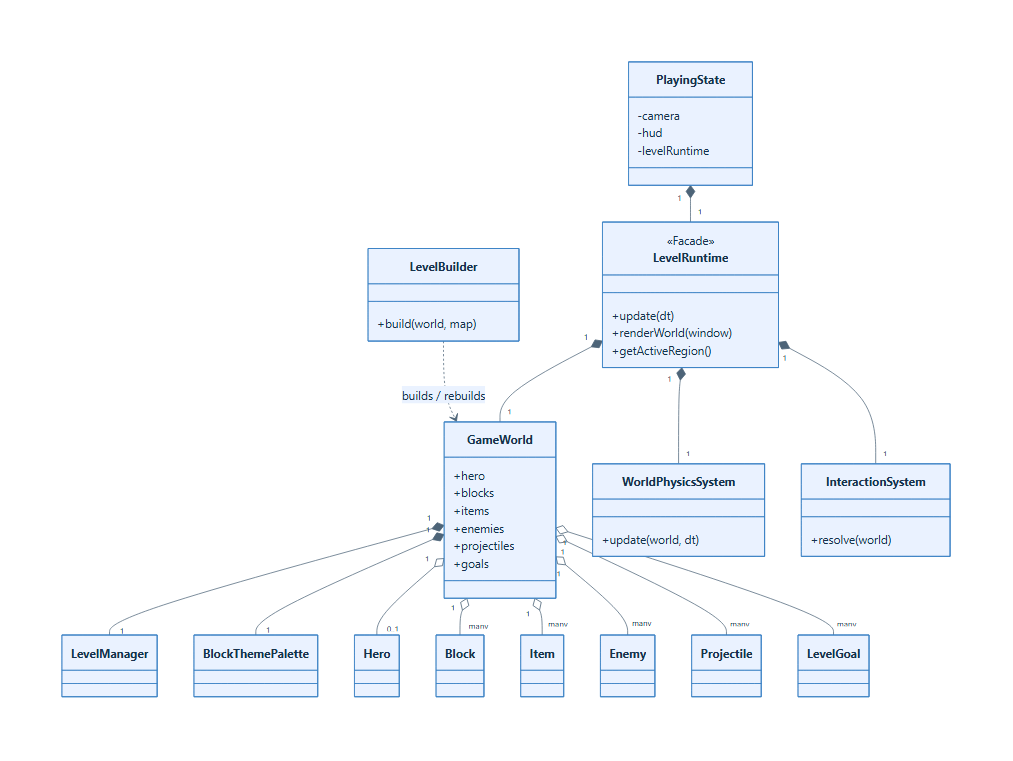
\includegraphics[width=0.95\textwidth,height=0.68\textheight,keepaspectratio]{img/diagrams/project-gameplay-facade.png}
\caption{Gameplay facade, systems, and ownership.}
\label{fig:gameplay-facade-diagram}
\end{figure}

\texttt{GameWorld} is the aggregate root for live gameplay data.  Its entity
collections use \texttt{std::unique\_ptr}; consequently, an entity has exactly
one owner and is destroyed automatically when removed or when the world is
cleared.  Systems receive a \texttt{GameWorld\&} temporarily and never take
ownership.  \texttt{SoundManager*} is explicitly non-owning because the audio
service belongs to \texttt{Game} and outlives every level.

\texttt{GameWorld::removeInactiveEntities} is the deferred cleanup point.
Entities mark themselves inactive, collected, or dead during update and
interaction passes; erasure occurs afterward, avoiding iterator invalidation.
For destroyed map blocks, the world also retains tile-coordinate pairs used by
persistence.  The world exposes a map-collider collection built from terrain
tiles for compatibility, while current high-frequency physics queries use the
\texttt{LevelManager} tile grid directly.

\subsubsection{Per-frame update order}

The order of a frame is part of the game's behavior:

\begin{enumerate}
    \item \texttt{PlayingState} obtains a newly pressed pipe direction and
    calls \texttt{LevelRuntime::update}.
    \item The runtime snapshots the room-bottom boundary of each active enemy.
    This prevents an enemy falling from a vertically stacked room from being
    incorrectly reassigned to the room below.
    \item Intrinsic updates run in the order Hero, Blocks, Items, Enemies, and
    Projectiles.  These updates handle input, state changes, animation,
    acceleration policy, timers, and spawning intent.
    \item \texttt{WorldPhysicsSystem} integrates velocity and resolves terrain
    and block collisions.
    \item \texttt{InteractionSystem} resolves cross-entity contacts and returns
    one score delta.
    \item The runtime enforces the live boss-arena boundary, attempts pipe
    travel, synchronizes the active region, applies hero/enemy fall deaths,
    culls out-of-world projectiles, and removes inactive entities.
    \item Back in \texttt{PlayingState}, score and coin changes are applied to
    the HUD; theme or invincibility music and the pixel-aligned camera are
    updated; then victory, time-out, defeat, and boss VFX are processed.
\end{enumerate}

Victory becomes authoritative once a goal has activated.  The hero enters
\texttt{CheerState}; after a short delay, a \texttt{VictoryState} overlay is
pushed.  Defeat restores the score/coin/lives snapshot from the start of the
attempt, removes one life, plays the player-down cue, and after two seconds
either retries through \texttt{TransitionState} or enters
\texttt{GameOverState}.

\subsubsection{Rendering order}

\texttt{PlayingState} installs the world camera and draws an underground black
backdrop when appropriate.  \texttt{LevelRuntime::renderWorld} then draws the
tile-map mesh, blocks in the active region, items, hero, enemies, and
projectiles.  Thor King phase-three overlays, lightning, fissures, and debris
are drawn by \texttt{PlayingState}.  Finally, the HUD is drawn in the default
window view so it remains screen-relative, and the default view is restored.

\subsection{Level and Map System}

\subsubsection{Data model and loading pipeline}

The level pipeline deliberately separates parsing, storage, rendering, and
gameplay construction.

\begin{figure}[htbp]
\centering
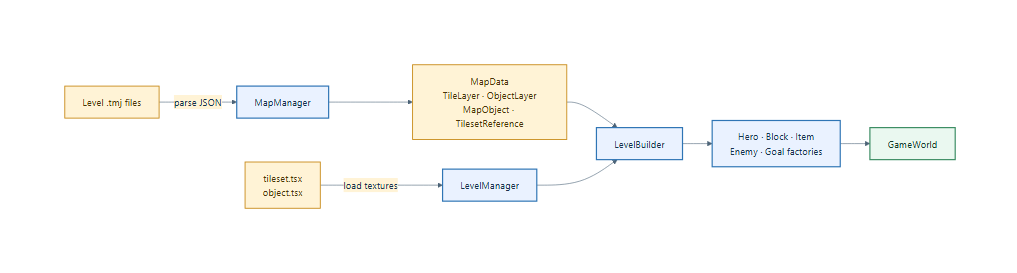
\includegraphics[width=0.96\textwidth,height=0.48\textheight,keepaspectratio]{img/diagrams/project-level-pipeline.png}
\caption{Data-driven level loading and construction pipeline.}
\label{fig:level-pipeline-diagram}
\end{figure}

\texttt{MapManager} parses map dimensions, tile size, tileset references,
visible tile layers, object layers, Tiled's modern \texttt{class} field with a
legacy \texttt{type} fallback, geometry, GIDs, and scalar custom properties.
\texttt{MapObject} retains all scalar properties in a string map and also
populates typed aliases such as target map, direction, contained item, theme,
and count.  \texttt{MapData} provides layer lookup, class queries, map pixel
dimensions, and matching pipe exits.

\texttt{LevelManager} owns the parsed \texttt{MapData}, the main and optional
object textures, and one pair of \texttt{sf::VertexArray} meshes per visible
tile layer.  At load time it resolves TSX image paths and converts all non-empty
tiles into texture-mapped quads.  Main-atlas and object-atlas quads are batched
separately, which reduces per-frame draw work compared with one sprite per tile.
It also supplies tile ID, solid-at-tile/pixel, interactive-tile, tile mutation,
and flexible object-query operations.  Pixel art uses nearest-neighbor sampling
and non-repeating textures to prevent atlas bleeding.

\subsubsection{Level construction}

\texttt{LevelBuilder::build} performs these steps:

\begin{enumerate}
    \item load the map and tilesets through \texttt{LevelManager};
    \item create the callback through which heroes and enemies transfer new
    projectiles into \texttt{GameWorld};
    \item find \texttt{Trigger/start} (with a legacy spawn fallback), create the
    selected hero through \texttt{HeroFactory}, and interpret the Tiled point as
    a foot-position anchor;
    \item create terrain rectangles for solid tiles;
    \item create Flag or Princess goal triggers from \texttt{Trigger/end};
    \item translate \texttt{Interactive} objects into bricks, question blocks,
    invisible blocks, ground coins, or a fallback flag, using factories and
    contained-item properties;
    \item match platform-up/platform-down spawners to unique
    \texttt{platform\_despawn} boundaries and construct \texttt{Lifter}
    platforms; and
    \item translate other \texttt{Spawner} objects into Goombas, Koopas,
    Witches, or Thor King.  Boss sound events are connected to the audio service.
\end{enumerate}

The construction code accepts selected legacy/case variants of object classes,
which protects existing maps during schema evolution.  New map schemas should
prefer one canonical spelling to reduce string-based branching.

\subsubsection{Playable regions, themes, pipes, and boss arena}

\texttt{LevelRuntime} caches valid \texttt{Trigger/playable\_region} rectangles.
The active region supplies the fall boundary, vertical camera anchor, block
theme, and block-render visibility.  Direct movement may switch between
side-by-side regions with vertical overlap; vertically stacked rooms are
switched explicitly through pipe destinations so falling into a pit cannot
accidentally enter the room below.  If no unique region contains the hero, the
runtime uses full map bounds and can infer a fallback theme from a boss arena.

Pipe entrances are \texttt{pipe\_in} triggers whose names match
\texttt{pipe\_out} objects.  Direction, hero alignment, grounded state, allowed
movement state, destination region, and a short cooldown are all checked.  The
destination point is interpreted as center-X and feet-Y, which keeps different
hero forms aligned.  The input direction is latched until release so a held key
does not immediately travel back through the exit.

Level 1-3 contains the current boss area.  A \texttt{boss\_arena} trigger gives
the arena metadata, and a boss spawner produces \texttt{ThorKing}.  While the
boss is alive, the runtime clamps the hero against the configured arena edge;
the restriction disappears after the boss dies.  The Princess goal represents
the final rescue endpoint.

\subsubsection{Current level catalogue}

\texttt{LevelCatalog.h} is a compile-time catalogue containing the displayed
number, world name, readiness status, map path, transition title, and compact
HUD world label for each level.  World 1-1 is an overworld with an underground
pipe room; world 1-2 is a larger multi-region level with several paired pipes
and moving lifters; world 1-3 is the boss level with Witches, Thor King, and a
Princess goal.  The associated data files are
\texttt{assets/maps/levels/1-1.tmj},
\texttt{assets/maps/levels/1-2.tmj}, and
\texttt{assets/maps/levels/1-3.tmj}; shared Tiled definitions are
\texttt{assets/maps/resources/tileset.tsx} and
\texttt{assets/maps/resources/object.tsx}.

\subsection{Character and Hero System}

\subsubsection{Base character abstraction}

\texttt{Character} is the abstract root for heroes and enemies.  It centralizes
position, velocity, hitbox shape, sprite, owned texture, animation controller,
life, facing direction, and grounded state.  Its polymorphic contract includes
update, render, damage, interaction, stomp/side-collision responses, speed,
health, touch damage, score value, and a stable type name.  The common setters
keep logical position, hitbox, and sprite synchronized.

\subsubsection{Hero class diagram}

\begin{figure}[htbp]
\centering
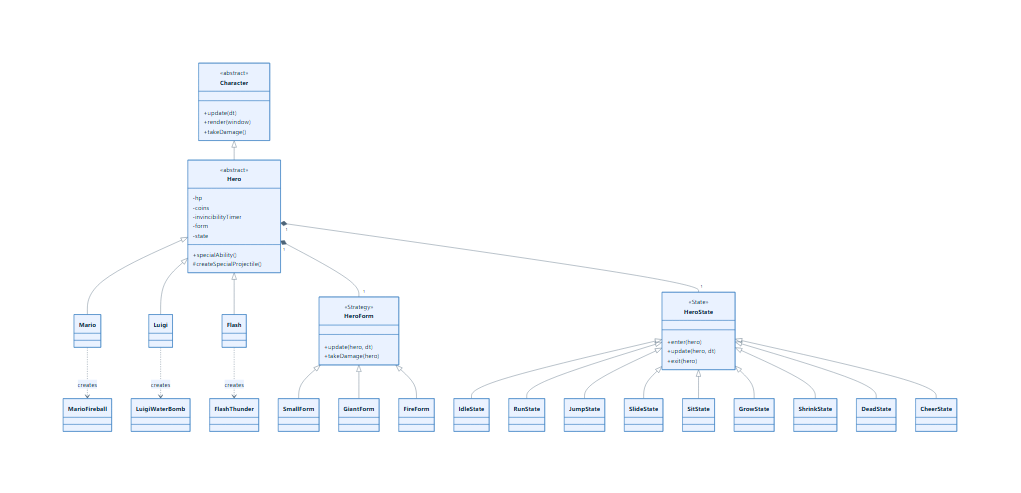
\includegraphics[width=0.99\textwidth,height=0.58\textheight,keepaspectratio]{img/diagrams/project-hero.png}
\caption{Character inheritance and the two orthogonal hero behavior axes.}
\label{fig:hero-class-diagram}
\end{figure}

\texttt{Hero} adds a form strategy, a movement state, base and special texture
paths, form-dependent sprite scales, override animation, invincibility and
Starman timers, coin and HP data, projectile spawning, and SFX callbacks.
\texttt{Hero::update} updates timers, synchronizes coordinates, delegates to
the form and state, and composes an animation key from form plus state (for
example, \texttt{GiantRun}).  Override animation supports a temporary special
attack without replacing the movement state.

Damage is form-dependent.  Small form dies, Giant form enters a Shrink state,
and Fire form first downgrades to Giant before using Giant's shrink behavior.
Invincibility frames prevent duplicate damage and render as blinking; Starman
invincibility uses color cycling and special music.  A falling hero who meets
the top portion of an enemy invokes \texttt{onStomped}, bounces upward, and
returns the enemy's score; other contact delegates to the enemy's side-collision
policy.

\subsubsection{Concrete heroes and forms}

\texttt{Mario}, \texttt{Luigi}, and \texttt{Flash} configure their own sprite
sheets and animation rectangles but share movement, form, and collision logic.
Their Factory Method creates different projectiles:

\begin{itemize}
    \item Mario's special form uses \texttt{FireMario.png}, a two-second
    cooldown, a special sound, and a horizontally launched fireball.
    \item Luigi's special form uses \texttt{KitsuneLuigi.png}, a three-second
    cooldown, and an upward-thrown water bomb that creates a splash.
    \item Flash's special form uses a processed \texttt{thunderflash2.png}, a
    $2.5$-second cooldown, and a fast thunder strike.  If the optional processed
    texture cannot be loaded, its animation table falls back to the base sheet.
\end{itemize}

A Mushroom only starts Small-to-Giant growth.  A Flower is collectible only by
an already powered hero and changes Giant to Fire; therefore Flash does not
become Thunder Flash merely by eating a Mushroom.  ``Fire'' is the shared
internal form name, although the visual and attack semantics are hero-specific.

\subsubsection{Hero movement state machine}

\begin{figure}[htbp]
\centering
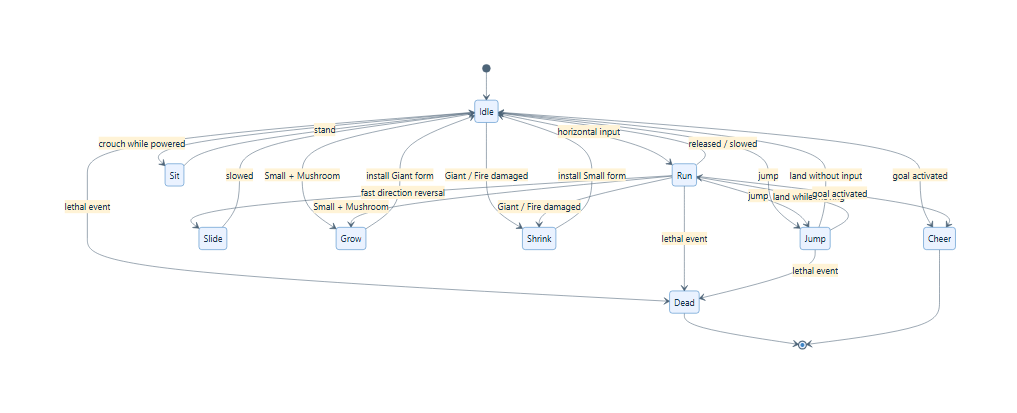
\includegraphics[width=0.98\textwidth,height=0.58\textheight,keepaspectratio]{img/diagrams/project-hero-state.png}
\caption{Principal transitions in the hero state machine.}
\label{fig:hero-state-machine}
\end{figure}

Idle, Run, Jump, Slide, and Sit own input-sensitive motion.  They use values
from \texttt{PhysicsConstants.h} for acceleration, friction, air control, jump
impulse, and fall speed.  Grow and Shrink are timed animation states.  Sit
temporarily changes a powered hero to a $32\times48$ hitbox and restores the
$32\times64$ standing hitbox on exit.  Dead owns defeat motion without terrain
collision, and Cheer locks velocity during level completion.

\subsection{Enemy and Boss System}

\subsubsection{Enemy hierarchy and composition}

\begin{figure}[htbp]
\centering
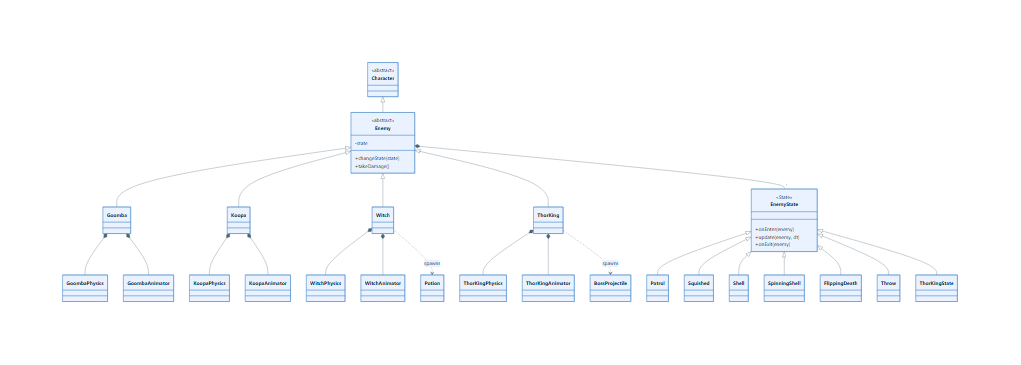
\includegraphics[width=0.99\textwidth,height=0.53\textheight,keepaspectratio]{img/diagrams/project-enemy.png}
\caption{Enemy inheritance, AI states, and composed helpers.}
\label{fig:enemy-class-diagram}
\end{figure}

\texttt{Enemy} supplies speed, health, patrol bounds, direction, sprite offset,
state timer, and the current \texttt{EnemyState}.  Patrol behavior checks bounds,
moves, and animates.  General collision responses damage the other character
or die when stomped, while subclasses refine those rules.

\texttt{Goomba} delegates movement/contact details to \texttt{GoombaPhysics}
and visual state to \texttt{GoombaAnimator}; a stomp uses a timed squished
state.  \texttt{Koopa} adds static and spinning shell modes, shell speed, wake
timer, kick cooldown, and shell-specific stomp and side-contact behavior.
Spinning shells can defeat other enemies through \texttt{InteractionSystem}.

\texttt{Witch} adds an attack cooldown and \texttt{ThrowState}.  At the attack
moment it creates an enemy-faction \texttt{Potion} through its callback.  A
potion follows gravity, becomes a wide temporary puddle on solid impact, and
can damage the hero during target interaction.

\subsubsection{Thor King boss}

\texttt{ThorKing} has three HP-based phases, increasing roll/fire behavior,
wall-bounce counters, a shot sequence, and a phase-three sky-launch cycle.
Its AI states separate patrol, crouch, rolling shell, vulnerable stun, fire
attack, and phase-change roar.  \texttt{ThorKingPhysics} owns boss collision and
damage transitions; \texttt{ThorKingAnimator} selects normal, enraged,
sky-meteor, and winged visual resources.  The boss publishes attack and defeat
sound events and can spawn straight or sky-drop attacks.  Its core HP and
counters are persisted, while transient AI resumes from a safe patrol state on
load.

This design keeps the general enemy contract usable by world systems.  The boss
is still an \texttt{Enemy}, so ordinary rendering, ownership, projectile target
selection, cleanup, and score rules apply.  Boss-specific behavior is isolated
to its class, helpers, AI states, arena code, and visual effects.

\subsection{Blocks and Items}

\subsubsection{Class diagram}

\begin{figure}[htbp]
\centering
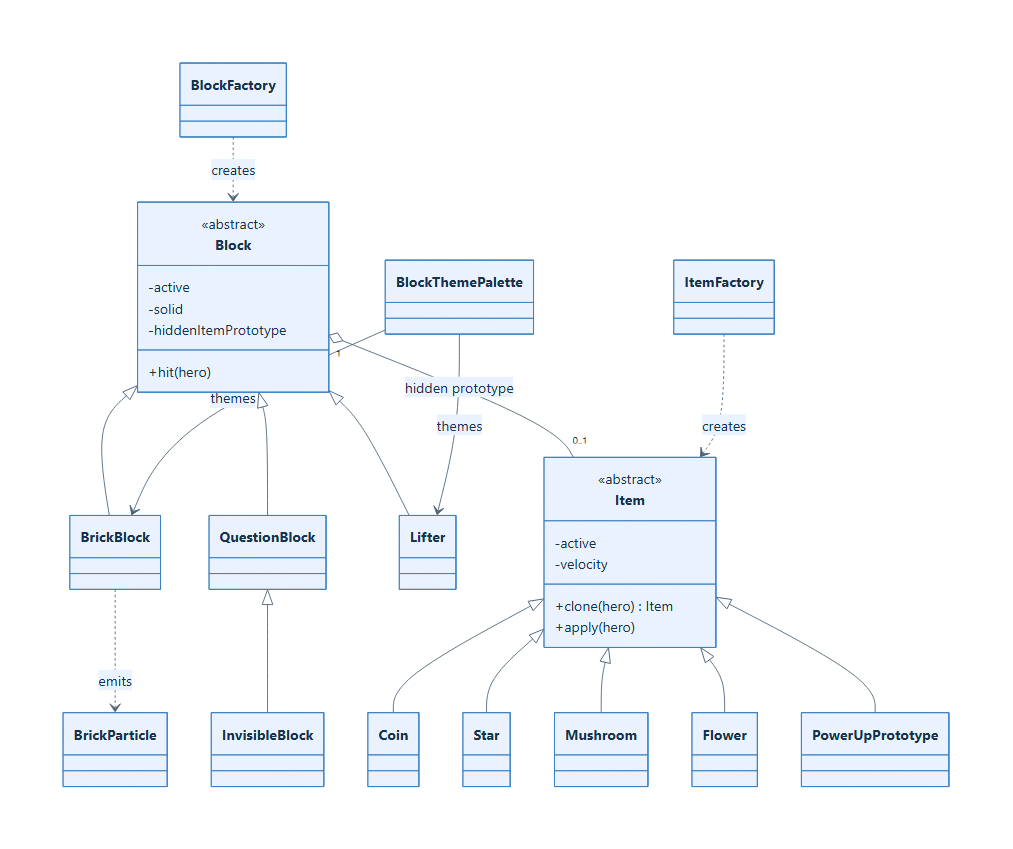
\includegraphics[width=0.97\textwidth,height=0.64\textheight,keepaspectratio]{img/diagrams/project-blocks-items.png}
\caption{Block, hidden-item Prototype, and collectible hierarchies.}
\label{fig:block-item-diagram}
\end{figure}

\texttt{Block} defines update, render, hit, lifetime, solidity, underside-hit
capability, and platform velocity.  It may own an item prototype and count.
\texttt{QuestionBlock} animates until its final hidden item is released and
then displays its empty frame.  \texttt{InvisibleBlock} derives from it but is
invisible and non-solid until hit from below.  \texttt{BrickBlock} either
releases its hidden item or, for Giant/Fire heroes, becomes four locally owned
\texttt{BrickParticle} records before deactivation.  \texttt{Lifter} is a
non-hittable solid platform that loops vertically between paired map bounds and
reports velocity so the physics system can carry a rider.

\texttt{BlockThemePalette} owns overworld, underground, and castle textures for
bricks and lifters.  The active playable-region theme selects the current
texture, so the same block objects can render correctly after pipe travel.
Blocks cache the bound theme but resynchronize during update/render.

\texttt{Item} defines spawning, cloning, collection, collision capability, and
movement data.  A ground Coin remains until collected; a block Coin is awarded
when cloned and performs a short bounce visual.  Mushroom emerges and begins
horizontal motion; Flower emerges without horizontal movement; Star emerges
and then bounces with temporary Starman invincibility on collection.
\texttt{PowerUpPrototype} chooses Mushroom or Flower at release time.  This
separation lets Tiled specify content and count while entity classes retain the
actual gameplay effects.

\subsection{Projectile System}

\begin{figure}[htbp]
\centering
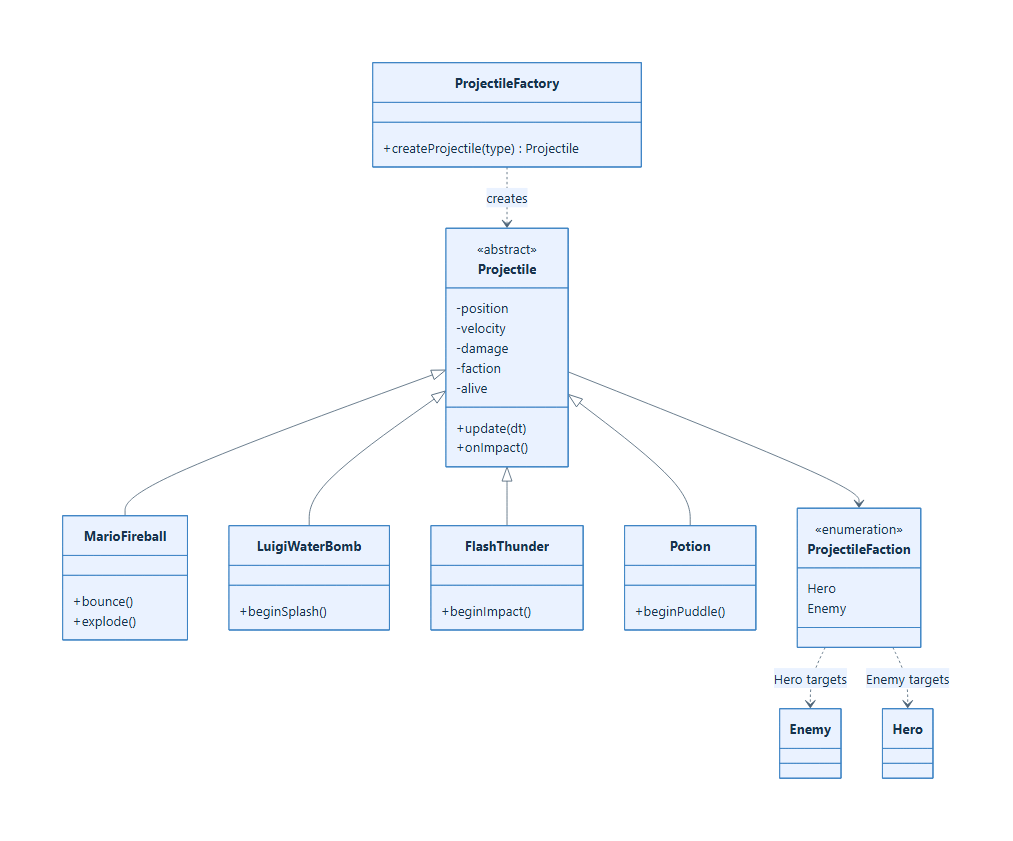
\includegraphics[width=0.92\textwidth,height=0.62\textheight,keepaspectratio]{img/diagrams/project-projectiles.png}
\caption{Unified projectile hierarchy and concrete phase behavior.}
\label{fig:projectile-class-diagram}
\end{figure}

The abstract \texttt{Projectile} contract separates intrinsic behavior from
world integration.  A projectile updates acceleration and phase timers, while
\texttt{WorldPhysicsSystem} integrates it only when
\texttt{usesWorldPhysics()} is true.  On collision, the system calls the
polymorphic \texttt{onSolidCollision}; target damage is handled through
\texttt{onHitTarget}.  \texttt{ProjectileFaction} prevents hero attacks from
targeting the hero and enemy attacks from targeting enemies.

\texttt{MarioFireball} follows gravity, bounces from floor contacts, and
explodes on walls or targets.  \texttt{LuigiWaterBomb} follows a strong arc and
expands into a one-frame damage splash.  \texttt{FlashThunder} travels without
gravity and expands into a pulsing impact strike.  Both area attacks retain a
set of already-hit character addresses and close their damage window after the
interaction pass.  \texttt{Potion} is the Witch's enemy projectile and becomes
a timed puddle.  \texttt{ProjectileFactory} reconstructs supported projectiles
from save strings while restoring velocity and faction.

\subsection{Physics and Interaction Systems}

\subsubsection{Class relationships}

\begin{figure}[htbp]
\centering
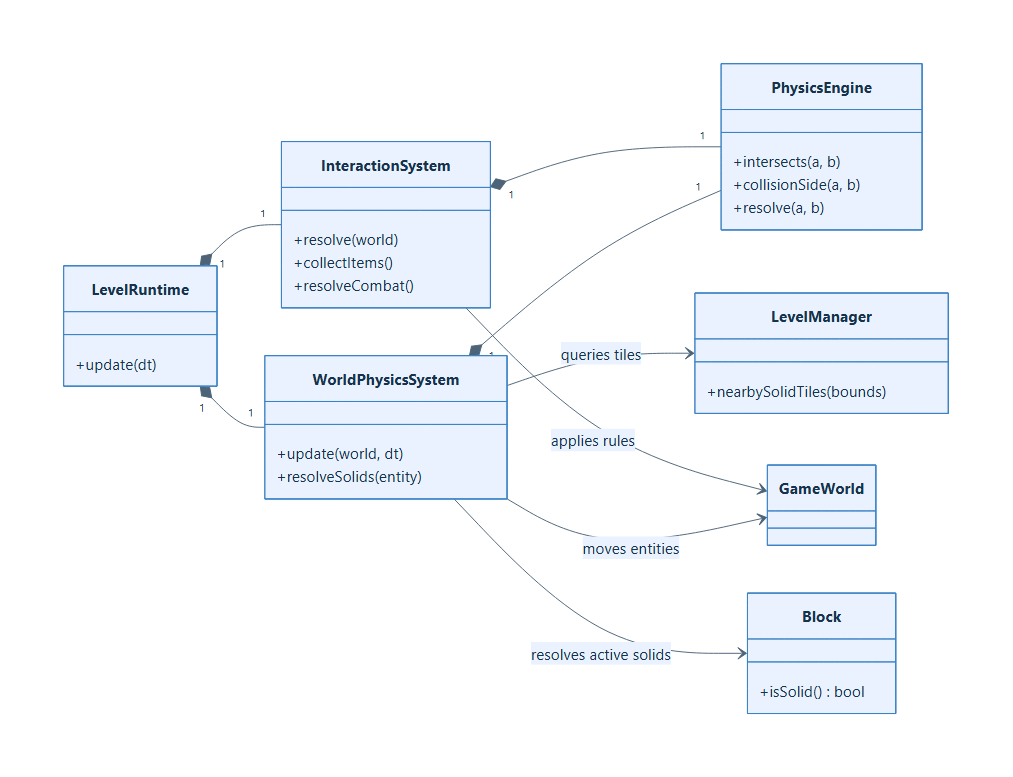
\includegraphics[width=0.96\textwidth,height=0.56\textheight,keepaspectratio]{img/diagrams/project-physics.png}
\caption{Separation between world collision and semantic interaction.}
\label{fig:physics-interaction-diagram}
\end{figure}

\texttt{PhysicsEngine} is the low-level axis-aligned bounding-box utility.  It
applies gravity, classifies a contact as Top, Bottom, Left, Right, or None, and
resolves X or Y overlap for either \texttt{sf::RectangleShape} or
\texttt{sf::FloatRect} obstacles.  \texttt{CollisionTypes.h} owns the shared
\texttt{SideType} enumeration.

\texttt{WorldPhysicsSystem} has four category-specific passes.  Hero collision
uses swept previous/proposed bounds to prevent tunneling and to select one
deterministic ceiling or landing surface.  It supports dynamic blocks, hidden
block hits, rider carry on downward lifters, grounded state, and separate X/Y
resolution.  Items integrate their velocity, land on solids, and reverse on
horizontal contacts.  Enemies receive gravity, collide with nearby terrain and
blocks, and notify or flip once on a wall.  Projectiles use their own gravity
policy and receive a polymorphic collision callback.

For performance, terrain collision enumerates only tile coordinates touched by
a swept query rectangle and asks \texttt{LevelManager::isSolidAtTile}.  It does
not scan every solid rectangle in a large level on every entity frame.  Dynamic
blocks remain a separate vector because their state, visibility, and position
can change.

\texttt{InteractionSystem} resolves semantic contacts in this order: hero-item,
spinning-shell/enemy, hero-enemy, projectile-target, and hero-goal.  It returns
one accumulated score delta.  Dead heroes and defeated/transitional enemies are
guarded consistently.  Hero area projectiles receive two target passes because
the first hit may expand their bounds; a per-frame set prevents resolving one
enemy twice.

Keeping the two systems separate is a major design decision.  A wall collision
changes geometry and velocity, while an item collection or enemy stomp changes
game semantics, score, audio, form, and lifetime.  Separating them makes the
per-frame order visible and prevents one monolithic collision routine from
knowing every concrete entity type.

\subsection{Goal and Level-Completion System}

\begin{figure}[htbp]
\centering
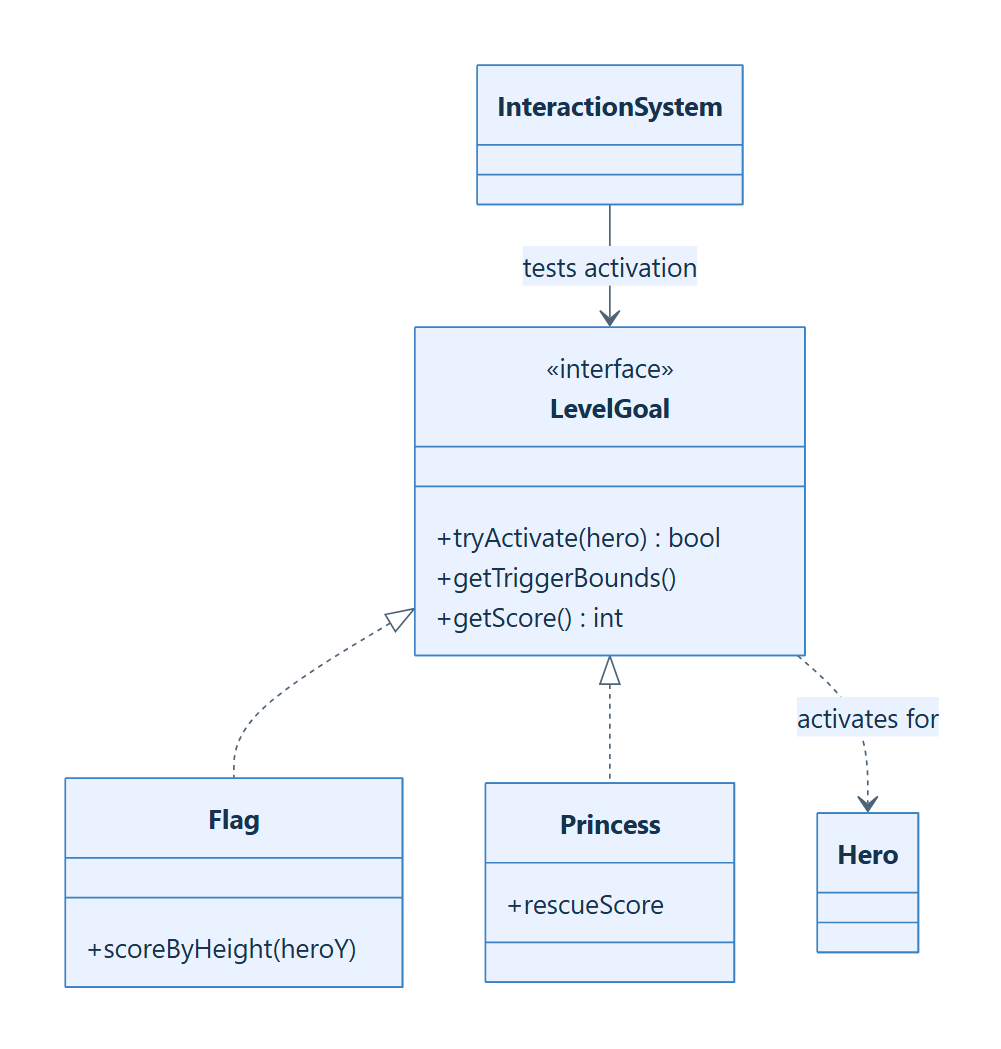
\includegraphics[width=0.66\textwidth,height=0.62\textheight,keepaspectratio]{img/diagrams/project-goals.png}
\caption{Polymorphic level goals.}
\label{fig:goal-class-diagram}
\end{figure}

\texttt{LevelGoal} is a non-rendering gameplay interface with a trigger,
activation state, score result, activation effect, and completion music.
\texttt{Flag} calculates a score between configured minimum and maximum values
from the hero's vertical contact position.  \texttt{Princess} awards a fixed
rescue score and selects its own completion cues.  The map remains responsible
for visual goal tiles; the goal object represents only semantic activation.

\texttt{InteractionSystem} attempts activation after all harmful interactions
for the frame and returns the award.  \texttt{PlayingState} observes the
activated goal, locks the hero in Cheer state, plays completion music, and opens
the Victory overlay.  This divides domain policy (whether/what a goal awards)
from screen policy (how completion is presented and where navigation goes).

\subsection{Save, Load, HUD, and Audio Services}

\subsubsection{Persistence class diagram and workflow}

\begin{figure}[htbp]
\centering
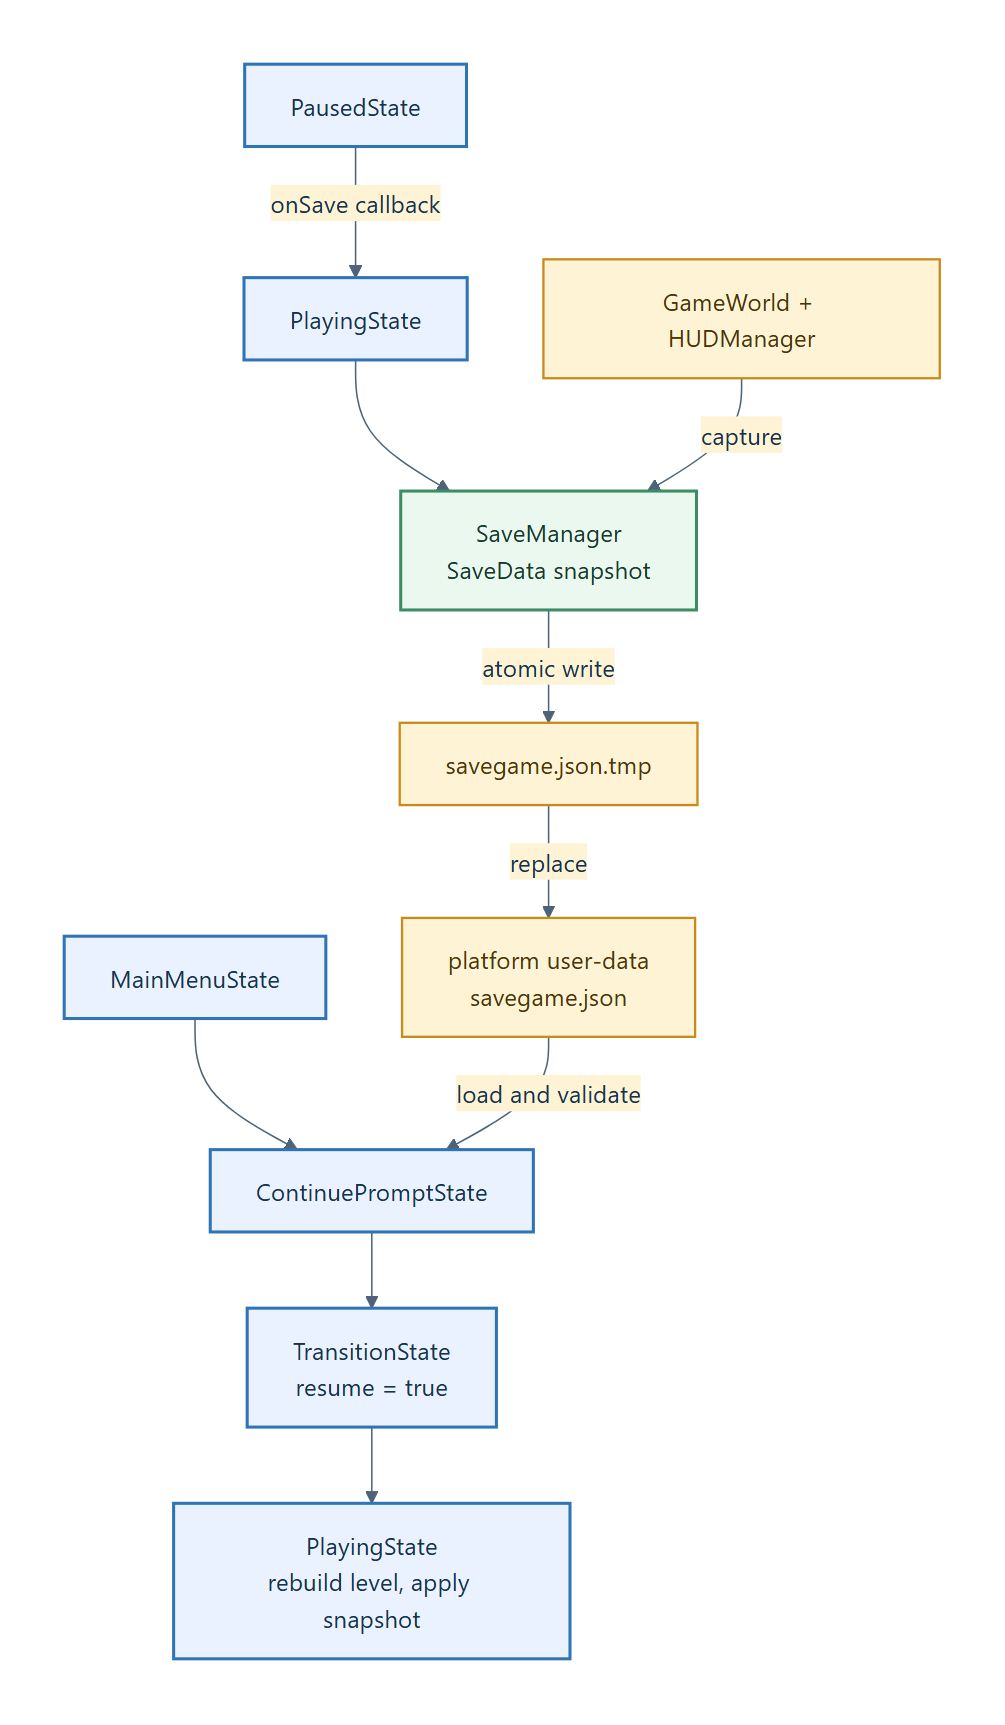
\includegraphics[width=0.66\textwidth,height=0.72\textheight,keepaspectratio]{img/diagrams/project-persistence.png}
\caption{Pause-save and menu-continue workflow.}
\label{fig:save-load-diagram}
\end{figure}

\texttt{SaveData} records map and tileset paths; hero position, HP, coins, type,
form, invincibility and Starman state; alive enemy position, velocity,
direction, health, grounded flag and AI state; additional Thor King counters;
hit and destroyed blocks; active item type and position; active projectile
type, position, velocity, and faction; and HUD score, coins, lives, and time.

\texttt{SaveManager::defaultSavePath} chooses a per-user application-data
directory on Windows, macOS, and other systems.  \texttt{existingSavePath}
also searches legacy working-directory locations.  Saving serializes JSON to a
temporary file, flushes and closes it, and then atomically replaces the target
where the operating system permits.  This is safer than truncating the only
valid save before a complete new snapshot is available.

Loading validates the JSON root, required level paths, hero object, supported
hero name, array types, and projectile faction before replacing in-memory
\texttt{SaveData}.  Continue first rebuilds the referenced level so static map
content and callbacks exist, then \texttt{applySaveToWorld} replaces the hero,
enemies, items, and projectiles through their factories, updates block/map
state, restores HUD values, and synchronizes camera region and music.

The persistence model is a snapshot, but not every transient variable is
captured.  Hero velocity, grounded/movement state, item velocity/spawn phase,
projectile lifetime/impact phase, lifter phase, activated goals, active region,
and exact boss AI timer are recomputed or reset.  This is a deliberate current
boundary: it produces a playable continuation but not bit-for-bit deterministic
resumption of the prior frame.  A future versioned save schema should add an
explicit format version and stable identifiers if exact restoration is needed.

\subsubsection{HUD}

\texttt{HUDManager} is both the model for score, coins, lives, world label, and
remaining time and an \texttt{sf::Drawable} view of those values.  Mutation
methods immediately regenerate the displayed strings.  \texttt{PlayingState}
applies score deltas from \texttt{LevelRuntime}, observes hero coin changes,
sets the compact world label from \texttt{LevelCatalog}, updates time, and
performs attempt/life restoration.  A shared pointer lets the same HUD survive
Transition, Playing, and Victory states.

\subsubsection{Audio}

\texttt{SoundManager} scans an SFX directory into named
\texttt{sf::SoundBuffer} objects, reuses a bounded pool of
\texttt{sf::Sound} channels, and streams one \texttt{sf::Music} track for BGM.
It supports independent SFX/BGM volumes and a master-volume operation.
\texttt{Game} owns it, settings modify it, screens select menu/game/result
music, and gameplay systems request effects directly or through callbacks.
Keeping the service above the level ensures music and volume survive state
replacement.

\subsection{Animation, Textures, and Other Utilities}

\begin{figure}[htbp]
\centering
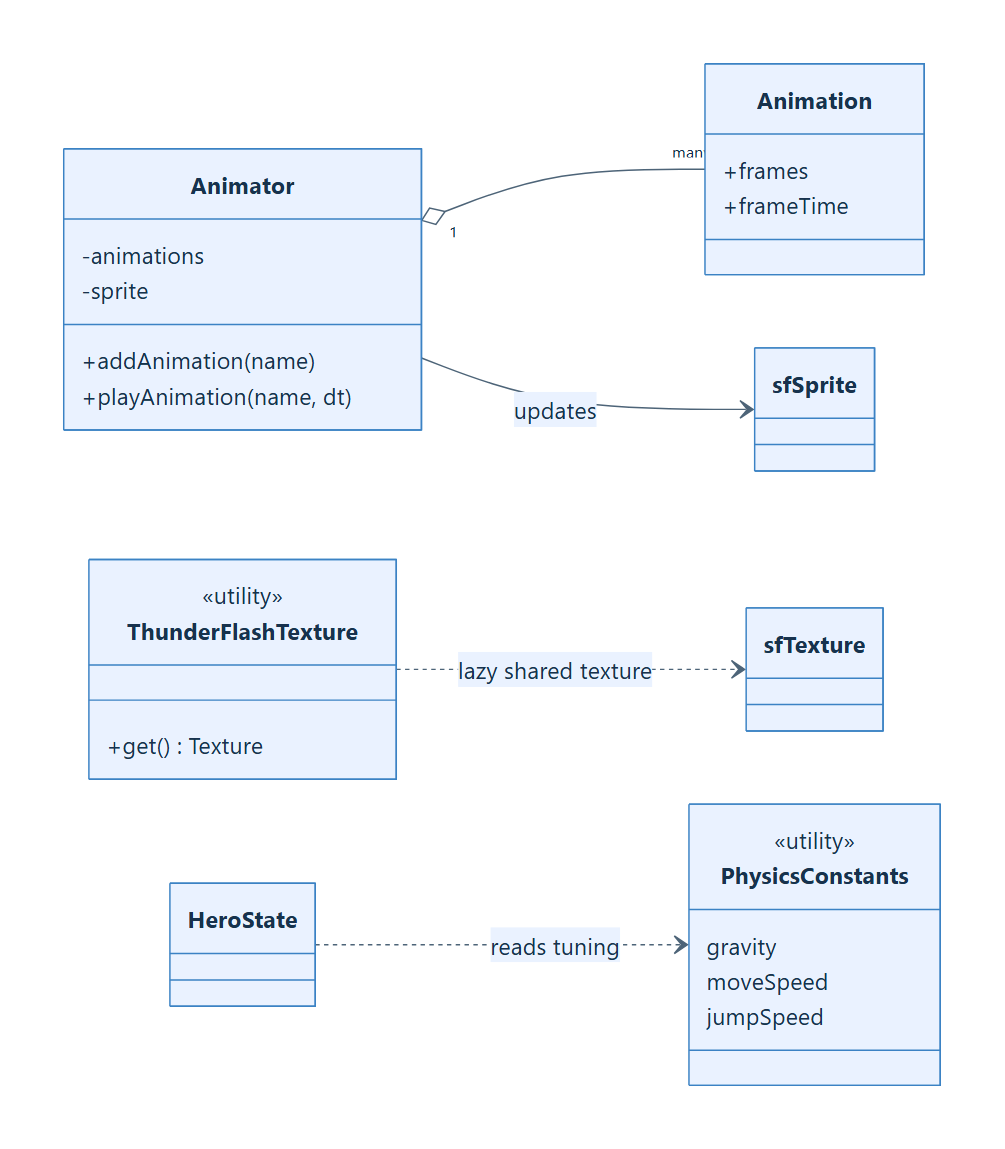
\includegraphics[width=0.88\textwidth,height=0.52\textheight,keepaspectratio]{img/diagrams/project-utilities.png}
\caption{Reusable animation and texture utilities.}
\label{fig:utility-diagram}
\end{figure}

\texttt{Animation} stores frame rectangles and duration, while
\texttt{Animator} stores named animations and mutates a referenced
\texttt{sf::Sprite}'s texture rectangle over time.  Characters, blocks, items,
and selected projectiles reuse this component.  Concrete hero constructors
register the combined form/state keys required by \texttt{Hero::update}.

\texttt{ThunderFlashTexture::get} lazily loads and transparency-processes the
Thunder Flash sheet and returns a shared non-owning texture pointer.  Lazy
creation ensures an SFML graphics context exists before the OpenGL resource is
initialized and avoids processing the same image for every Flash-related
object.  \texttt{PhysicsConstants.h} centralizes hero movement tuning rather
than scattering values across movement states.

\subsection{Ownership, Coupling, and Extension Rationale}

The principal ownership rules are:

\begin{itemize}
    \item \texttt{Game} uniquely owns screen states and the audio service;
    \item \texttt{PlayingState} owns its \texttt{LevelRuntime} by value and
    shares one HUD across related states;
    \item \texttt{LevelRuntime} owns the world and systems by value;
    \item \texttt{GameWorld} uniquely owns the hero and all entity instances;
    \item \texttt{Hero} uniquely owns its form and movement state;
    \item \texttt{Enemy} uniquely owns its AI state;
    \item \texttt{Block} uniquely owns a hidden item prototype; and
    \item pointers to \texttt{SoundManager}, references to
    \texttt{BlockThemePalette}, and callback captures are non-owning.
\end{itemize}

This arrangement avoids cycles among smart pointers.  Spawn callbacks transfer
\texttt{unique\_ptr} ownership outward to the world, while notifications carry
events without exposing the world's internals.  Abstract bases are used where
the world needs uniform lifetime/update/render behavior.  Capability methods
such as \texttt{isSolid}, \texttt{canBeHitFromBelow},
\texttt{usesWorldPhysics}, and \texttt{onSolidCollision} are preferred over
concrete casts; casts remain for explicitly boss-specific behavior.

To add a hero, implement the concrete texture/animation table and special
projectile Factory Method, add a \texttt{HeroType} and factory mapping, then add
selection UI and save parsing.  To add an enemy, implement its state/physics/
animation requirements, add an enemy factory mapping, recognize its Tiled
spawner class, and add save support if it has unique transient data.  To add a
level, add the TMJ/TSX-compatible data, a \texttt{LevelCatalog} entry, valid
start/end triggers, and only those playable regions/pipes/boss markers intended
by the design.  These extension paths explain why construction, simulation,
and presentation are separated.

\subsection{Current Constraints and Improvement Opportunities}

The current design is coherent but has several explicit trade-offs:

\begin{itemize}
    \item entity, state, form, animation, Tiled-class, and audio identifiers are
    strings in multiple boundaries; centralized constants or typed IDs would
    reduce spelling-dependent behavior;
    \item Observer behavior is callback/direct-notification based rather than a
    reusable typed event system, and coin synchronization is currently polled;
    \item some constructors load textures independently, so a general asset
    cache would reduce duplicate I/O and texture memory;
    \item state updates and most interactions use linear scans; spinning-shell
    and projectile targeting can become quadratic with many enemies, so spatial
    partitioning would be the next scaling step;
    \item the level builder still materializes a rectangle for each solid tile
    even though active collision uses nearby tile-grid queries; removing or
    repurposing the redundant collection would reduce large-level memory and
    load work;
    \item boss VFX and debug phase/form hotkeys are currently in
    \texttt{PlayingState}; a dedicated boss encounter/presentation component
    would keep the scene controller smaller;
    \item save files have validation but no schema version or migration layer;
    and
    \item there is no project-owned automated test target in the current CMake
    configuration, so regression verification depends on builds and manual play.
\end{itemize}

These are evolution points, not reasons to collapse the present subsystem
boundaries.  Improvements should preserve world ownership, deferred cleanup,
the physics/interaction split, and state-transition safety.

\subsection{Build and Deployment Structure}

\texttt{CMakeLists.txt} declares a C++17 executable named
\texttt{Custom2DPlatformer}, obtains SFML 2.6.1 through CMake FetchContent,
recursively includes project source/header directories, and links SFML graphics,
window, system, and audio libraries statically.  A post-build command copies
the complete \texttt{assets} directory beside the executable.  On Windows it
also copies the architecture-correct \texttt{openal32.dll}, because SFML's
OpenAL audio backend remains a runtime dependency even when SFML itself is
linked statically.  This explains why asset paths are relative to the executable
working directory and why both assets and OpenAL must accompany a distributed
binary.

\subsection{Complete Source-File Catalogue}
\label{subsec:source-file-catalogue}

This catalogue accounts for every current project-owned C++ header and source
file.  A notation such as \path{X.h / X.cpp} denotes the declaration and its
implementation at the corresponding \path{include} and \path{src} paths.
Interface-only headers are identified explicitly.

\begingroup
\Urlmuskip=0mu plus 1mu\relax

\subsubsection{Bootstrap and core application}

\begin{itemize}
    \item \path{src/main.cpp}: process entry point and Windows I/O
    compatibility shim.
    \item \path{include/Core/Game.h} /
    \path{src/Core/Game.cpp}: singleton application object, loop, audio,
    state stack, selection, and deferred transitions.
    \item \path{include/Core/State.h}: abstract screen-state interface.
    \item \path{include/Core/CollisionTypes.h}: shared collision-side enum.
    \item \path{include/Core/PhysicsEngine.h} /
    \path{src/Core/PhysicsEngine.cpp}: AABB collision and resolution helpers.
    \item \path{include/Core/LevelCatalog.h}: compile-time level metadata and
    next-level lookup.
\end{itemize}

\subsubsection{Screen states}

\begin{itemize}
    \item \path{include/Core/MainMenuState.h} /
    \path{src/Core/MainMenuState.cpp}.
    \item \path{include/Core/ContinuePromptState.h} /
    \path{src/Core/ContinuePromptState.cpp}.
    \item \path{include/Core/CharacterSelectState.h} /
    \path{src/Core/CharacterSelectState.cpp}.
    \item \path{include/Core/LevelSelectState.h} /
    \path{src/Core/LevelSelectState.cpp}.
    \item \path{include/Core/GuideState.h} /
    \path{src/Core/GuideState.cpp}.
    \item \path{include/Core/SettingsState.h} /
    \path{src/Core/SettingsState.cpp}.
    \item \path{include/Core/TransitionState.h} /
    \path{src/Core/TransitionState.cpp}.
    \item \path{include/Core/PlayingState.h} /
    \path{src/Core/PlayingState.cpp}.
    \item \path{include/Core/PausedState.h} /
    \path{src/Core/PausedState.cpp}.
    \item \path{include/Core/VictoryState.h} /
    \path{src/Core/VictoryState.cpp}.
    \item \path{include/Core/GameOverState.h} /
    \path{src/Core/GameOverState.cpp}.
\end{itemize}

\subsubsection{Gameplay runtime}

\begin{itemize}
    \item \path{include/Core/Gameplay/GameWorld.h} /
    \path{src/Core/Gameplay/GameWorld.cpp}: world ownership and cleanup.
    \item \path{include/Core/Gameplay/LevelRuntime.h} /
    \path{src/Core/Gameplay/LevelRuntime.cpp}: live-level facade and frame
    pipeline.
    \item \path{include/Core/Gameplay/LevelBuilder.h} /
    \path{src/Core/Gameplay/LevelBuilder.cpp}: map-to-world construction.
    \item \path{include/Core/Gameplay/WorldPhysicsSystem.h} /
    \path{src/Core/Gameplay/WorldPhysicsSystem.cpp}: movement and solid
    collision.
    \item \path{include/Core/Gameplay/InteractionSystem.h} /
    \path{src/Core/Gameplay/InteractionSystem.cpp}: semantic contacts and
    scoring.
    \item \path{include/Core/Gameplay/BlockThemePalette.h} /
    \path{src/Core/Gameplay/BlockThemePalette.cpp}: region-sensitive block
    textures.
\end{itemize}

\subsubsection{Character and hero files}

\begin{itemize}
    \item \path{include/Entities/Character/Character.h} /
    \path{src/Entities/Character/Character.cpp}: abstract character root.
    \item \path{include/Entities/Character/Hero/Hero.h} /
    \path{src/Entities/Character/Hero/Hero.cpp}: common hero behavior.
    \item \path{include/Entities/Character/Hero/HeroFactory.h} /
    \path{src/Entities/Character/Hero/HeroFactory.cpp}: hero construction.
    \item \path{include/Entities/Character/Hero/Mario.h} /
    \path{src/Entities/Character/Hero/Mario.cpp};
    \path{include/Entities/Character/Hero/Luigi.h} /
    \path{src/Entities/Character/Hero/Luigi.cpp}; and
    \path{include/Entities/Character/Hero/Flash.h} /
    \path{src/Entities/Character/Hero/Flash.cpp}: concrete heroes.
\end{itemize}

\subsubsection{Hero form and movement-state files}

\begin{itemize}
    \item \path{include/Entities/Character/Hero/HeroForm/HeroForm.h}:
    abstract form strategy.
    \item \path{include/Entities/Character/Hero/HeroForm/SmallForm.h} /
    \path{src/Entities/Character/Hero/HeroForm/SmallForm.cpp}.
    \item \path{include/Entities/Character/Hero/HeroForm/GiantForm.h} /
    \path{src/Entities/Character/Hero/HeroForm/GiantForm.cpp}.
    \item \path{include/Entities/Character/Hero/HeroForm/FireForm.h} /
    \path{src/Entities/Character/Hero/HeroForm/FireForm.cpp}.
    \item \path{include/Entities/Character/Hero/HeroState/HeroState.h}:
    abstract movement-state interface.
    \item \path{include/Entities/Character/Hero/HeroState/IdleState.h} /
    \path{src/Entities/Character/Hero/HeroState/IdleState.cpp}.
    \item \path{include/Entities/Character/Hero/HeroState/RunState.h} /
    \path{src/Entities/Character/Hero/HeroState/RunState.cpp}.
    \item \path{include/Entities/Character/Hero/HeroState/JumpState.h} /
    \path{src/Entities/Character/Hero/HeroState/JumpState.cpp}.
    \item \path{include/Entities/Character/Hero/HeroState/SlideState.h} /
    \path{src/Entities/Character/Hero/HeroState/SlideState.cpp}.
    \item \path{include/Entities/Character/Hero/HeroState/SitState.h} /
    \path{src/Entities/Character/Hero/HeroState/SitState.cpp}.
    \item \path{include/Entities/Character/Hero/HeroState/GrowState.h} /
    \path{src/Entities/Character/Hero/HeroState/GrowState.cpp}.
    \item \path{include/Entities/Character/Hero/HeroState/ShrinkState.h} /
    \path{src/Entities/Character/Hero/HeroState/ShrinkState.cpp}.
    \item \path{include/Entities/Character/Hero/HeroState/DeadState.h} /
    \path{src/Entities/Character/Hero/HeroState/DeadState.cpp}.
    \item \path{include/Entities/Character/Hero/HeroState/CheerState.h} /
    \path{src/Entities/Character/Hero/HeroState/CheerState.cpp}.
\end{itemize}

\subsubsection{Enemy and boss files}

\begin{itemize}
    \item \path{include/Entities/Character/Enemy/Enemy.h} /
    \path{src/Entities/Character/Enemy/Enemy.cpp}: common enemy entity.
    \item \path{include/Entities/Character/Enemy/EnemyFactory.h} /
    \path{src/Entities/Character/Enemy/EnemyFactory.cpp}: static and
    polymorphic enemy factories.
    \item \path{include/Entities/Character/Enemy/EnemyState.h} /
    \path{src/Entities/Character/Enemy/EnemyState.cpp}: common AI states.
    \item \path{include/Entities/Character/Enemy/EnemyStateFactory.h} /
    \path{src/Entities/Character/Enemy/EnemyStateFactory.cpp}: saved-state
    reconstruction.
    \item \path{include/Entities/Character/Enemy/Goomba.h} /
    \path{src/Entities/Character/Enemy/Goomba.cpp},
    \path{include/Entities/Character/Enemy/GoombaPhysics.h} /
    \path{src/Entities/Character/Enemy/GoombaPhysics.cpp}, and
    \path{include/Entities/Character/Enemy/GoombaAnimator.h} /
    \path{src/Entities/Character/Enemy/GoombaAnimator.cpp}.
    \item \path{include/Entities/Character/Enemy/Koopa.h} /
    \path{src/Entities/Character/Enemy/Koopa.cpp},
    \path{include/Entities/Character/Enemy/KoopaPhysics.h} /
    \path{src/Entities/Character/Enemy/KoopaPhysics.cpp}, and
    \path{include/Entities/Character/Enemy/KoopaAnimator.h} /
    \path{src/Entities/Character/Enemy/KoopaAnimator.cpp}.
    \item \path{include/Entities/Character/Enemy/Witch.h} /
    \path{src/Entities/Character/Enemy/Witch.cpp},
    \path{include/Entities/Character/Enemy/WitchPhysics.h} /
    \path{src/Entities/Character/Enemy/WitchPhysics.cpp}, and
    \path{include/Entities/Character/Enemy/WitchAnimator.h} /
    \path{src/Entities/Character/Enemy/WitchAnimator.cpp}.
    \item \path{include/Entities/Character/Enemy/ThorKing.h} /
    \path{src/Entities/Character/Enemy/ThorKing.cpp},
    \path{include/Entities/Character/Enemy/ThorKingPhysics.h} /
    \path{src/Entities/Character/Enemy/ThorKingPhysics.cpp},
    \path{include/Entities/Character/Enemy/ThorKingAnimator.h} /
    \path{src/Entities/Character/Enemy/ThorKingAnimator.cpp}, and
    \path{include/Entities/Character/Enemy/ThorKingState.h} /
    \path{src/Entities/Character/Enemy/ThorKingState.cpp}.
    \item \path{include/Entities/Character/Enemy/Projectile.h} /
    \path{src/Entities/Character/Enemy/Projectile.cpp}: shared projectile
    abstraction retained in the enemy directory for historical compatibility.
    \item \path{include/Entities/Character/Enemy/Potion.h} /
    \path{src/Entities/Character/Enemy/Potion.cpp}: Witch projectile.
\end{itemize}

\subsubsection{Block files}

\begin{itemize}
    \item \path{include/Entities/Block/Block.h} /
    \path{src/Entities/Block/Block.cpp} and
    \path{include/Entities/Block/BlockFactory.h} /
    \path{src/Entities/Block/BlockFactory.cpp}.
    \item \path{include/Entities/Block/BrickBlock.h} /
    \path{src/Entities/Block/BrickBlock.cpp} and the declaration-only
    \path{include/Entities/Block/BrickParticle.h}.
    \item \path{include/Entities/Block/QuestionBlock.h} /
    \path{src/Entities/Block/QuestionBlock.cpp}.
    \item \path{include/Entities/Block/InvisibleBlock.h} /
    \path{src/Entities/Block/InvisibleBlock.cpp}.
    \item \path{include/Entities/Block/Lifter.h} /
    \path{src/Entities/Block/Lifter.cpp}.
\end{itemize}

\subsubsection{Item files}

\begin{itemize}
    \item \path{include/Entities/Item/Item.h} /
    \path{src/Entities/Item/Item.cpp} and
    \path{include/Entities/Item/ItemFactory.h} /
    \path{src/Entities/Item/ItemFactory.cpp}.
    \item \path{include/Entities/Item/PowerUpPrototype.h} /
    \path{src/Entities/Item/PowerUpPrototype.cpp}.
    \item \path{include/Entities/Item/Coin.h} /
    \path{src/Entities/Item/Coin.cpp}.
    \item \path{include/Entities/Item/Mushroom.h} /
    \path{src/Entities/Item/Mushroom.cpp}.
    \item \path{include/Entities/Item/Flower.h} /
    \path{src/Entities/Item/Flower.cpp}.
    \item \path{include/Entities/Item/Star.h} /
    \path{src/Entities/Item/Star.cpp}.
\end{itemize}

\subsubsection{Hero projectile and goal files}

\begin{itemize}
    \item \path{include/Entities/Projectile/ProjectileFactory.h} /
    \path{src/Entities/Projectile/ProjectileFactory.cpp}.
    \item \path{include/Entities/Projectile/MarioFireball.h} /
    \path{src/Entities/Projectile/MarioFireball.cpp}.
    \item \path{include/Entities/Projectile/LuigiWaterBomb.h} /
    \path{src/Entities/Projectile/LuigiWaterBomb.cpp}.
    \item \path{include/Entities/Projectile/FlashThunder.h} /
    \path{src/Entities/Projectile/FlashThunder.cpp}.
    \item \path{include/Entities/Goal/LevelGoal.h}: goal interface.
    \item \path{include/Entities/Goal/Flag.h} /
    \path{src/Entities/Goal/Flag.cpp}.
    \item \path{include/Entities/Goal/Princess.h} /
    \path{src/Entities/Goal/Princess.cpp}.
\end{itemize}

\subsubsection{Manager and utility files}

\begin{itemize}
    \item \path{include/Managers/MapData.hpp} /
    \path{src/Managers/MapData.cpp} and
    \path{include/Managers/MapManager.hpp} /
    \path{src/Managers/MapManager.cpp}.
    \item \path{include/Managers/LevelManager.hpp} /
    \path{src/Managers/LevelManager.cpp}.
    \item \path{include/Managers/SaveManager.hpp} /
    \path{src/Managers/SaveManager.cpp}.
    \item \path{include/Managers/HUDManager.hpp} /
    \path{src/Managers/HUDManager.cpp}.
    \item \path{include/Managers/SoundManager.hpp} /
    \path{src/Managers/SoundManager.cpp}.
    \item \path{include/Utilities/Animator.h} /
    \path{src/Utilities/Animator.cpp}.
    \item \path{include/Utilities/PhysicsConstants.h}: shared movement
    constants.
    \item \path{include/Utilities/ThunderFlashTexture.h} /
    \path{src/Utilities/ThunderFlashTexture.cpp}: shared processed texture.
\end{itemize}

Finally, \path{include/nlohmann/json.hpp} and
\path{include/nlohmann/json_fwd.hpp} are vendored third-party headers rather
than project-authored domain classes.  They are nevertheless part of the build:
\path{MapManager} uses them to parse TMJ files and \path{SaveManager} uses
them to serialize and validate save snapshots.  \path{CMakeLists.txt} is the
project's build description and completes the code/build inventory.
\par
\endgroup
\par
\endgroup
